\documentclass[12pt,a4paper]{article}
\usepackage{geometry}
\geometry{a4paper, left=2.5cm, right=2.5cm, top=2.5cm, bottom=2.5cm} % 设置页面边距
\usepackage{ctex} % 中文支持 (使用 XeLaTeX 编译器)
\usepackage{multirow}%表格多行合并
\usepackage{diagbox} % 在导言区添加
\usepackage{graphicx} % 插入图片
\usepackage{array}
\usepackage{float} % 图片浮动支持
\usepackage{amsmath, amssymb, amsthm} % 数学符号
\usepackage{booktabs} % 专业表格
\usepackage{listings} % 代码高亮
\usepackage{color} % 代码颜色
\usepackage[table,xcdraw]{xcolor}
\usepackage{hyperref} % 超链接
\usepackage[numbers]{natbib}
\hypersetup{colorlinks, urlcolor=blue, citecolor=blue, linkcolor=blue} % 链接颜色
\renewcommand{\parallel}{\mathrel{/ \mskip-4mu /}}
% 设置代码高亮
\definecolor{bluekeywords}{rgb}{0.13,0.13,1}
\definecolor{greencomments}{rgb}{0,0.5,0}
\definecolor{redstrings}{rgb}{0.9,0,0}
\lstset{
	language=Matlab, % 设置为 MATLAB
	basicstyle=\small,
	keywordstyle=\color{bluekeywords},
	commentstyle=\color{greencomments},
	stringstyle=\color{redstrings},
	showstringspaces=false,
	frame=single,
	numbers=left,
	numberstyle=\tiny,
	numbersep=5pt,
	xleftmargin=0.1cm,
	xrightmargin=0cm,
	aboveskip=0.5cm,
	belowskip=0.5cm,
	columns=fullflexible,
	backgroundcolor=\color{white},
	breaklines=true
}

% 设置标题格式
%\title{\textbf{实验报告:[实验标题]}}
%\author{[你的名字]}
%\date{\today}

\begin{document}
	
	% 封面页
	\begin{titlepage}
		\centering
		{\Huge 实验报告}\par\vspace{1.5cm}
		{\Large 实验名称}\par\vspace{1cm}
		{\large 指导教师:xxx}\par\vspace{0.5cm}
		{\large ASwallow}\par\vspace{0.5cm}
		{\large xx大学}\par\vspace{5cm}
		
		\large Experiment Date: \hspace{4cm} \today\par\vspace{0.5cm} % 实验日期
		\rule{10cm}{0.4pt} \\
		\textbf{实验报告签字} 
	\end{titlepage}
	
	\tableofcontents
	\newpage
	
	\section{实验目的}
	\begin{itemize}
		\item 1
		\item 2
	\end{itemize}
	
	\section{主要实验仪器}
	\begin{itemize}
		\item [仪器1]:1
		\item [仪器2]:2
	\end{itemize}
	
	\section{实验原理}
	
	
	\begin{equation}
		\rho(\theta)=\rho_\perp+(\rho_{\parallel}-\rho_\perp )\cos^2\theta
	\end{equation}
	
	其中,\(\rho_\perp\),\(\rho_{\parallel}\)表示电流垂直于磁化强度和平行于磁化强度的电阻率,\(\theta\)表示电流和磁化强度的夹角。
	
	参考内部电路图\cite{wang2002新型磁阻传感器在地磁场测量中的应用}得到其输出电压为
	\begin{figure}[H]
		\centering
		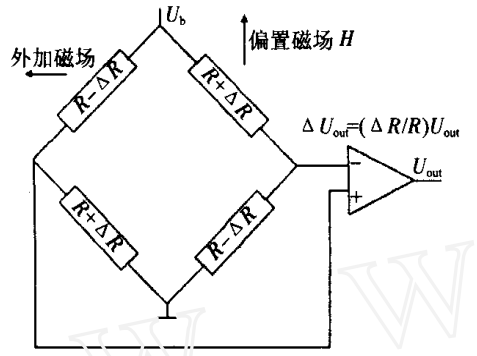
\includegraphics[width=0.6\textwidth]{dianlu.png}
		\caption{磁阻传感器内部部分电路}
		\label{fig:0}
	\end{figure}
	\begin{equation}
		U_{out}=\frac{R+\Delta R}{2R}\cdot U_b-\frac{R-\Delta R}{2R}\cdot U_b=\frac{\Delta R}{R}\cdot U_b
	\end{equation}
	
	如果确定一定的工作电压,则有
	\begin{equation}
		U_{out}=U_0+KB
	\end{equation}
	其中,\(K\)为仪器的灵敏度,\(B\)为待测感应强度,\(U_0\)为外加磁场为0的传感器输出量。
	
	亥姆霍兹线圈公共轴线中心点位置处的磁感应强度为
	\begin{equation}
		B=\frac{\mu_0NI}{R}\frac{8}{5^{3/2}}
	\end{equation}
	取\(N\)为500,\(R\)为亥姆霍兹线圈半径。
	\section{实验步骤}
	\begin{itemize}
		\item 1
		\item 2
		\item 3

	\end{itemize}
	
	
	
	\section{实验数据}
	
	
	
	
	\begin{table}[h]
		\centering
		\caption{磁阻传感器灵敏度}
		\label{tab:bea}
		\begin{tabular}{|c|c|c|c|c|}
			\hline
			\multirow{2}{*}{励磁电流 $I/mA$} & \multirow{2}{*}{磁感应强度 $B/10^{-4}T$} & \multicolumn{3}{c|}{$U/mV$} \\ \cline{3-5} 
			&  & 正向 $U_1/mV$ & 反向 $U_2/mV$ & 平均 $|U|/mV$ \\ 
			\hline
			&  &  &  &  \\ 
			\hline
			&  &  &  &  \\ 
			\hline
			&  &  &  &  \\ 
			\hline
			&  &  &  &  \\ 
			\hline
		\end{tabular}
	\end{table}
	\begin{table}[h]
		\centering
		\caption{磁倾角 $\beta$ 的测量}
		\label{tab:beta}
		\begin{tabular}{|c|c|c|c|c|c|c|c|c|c|c|c|c|c|c|}
			\hline
			
			$\beta$ &  &  &	&	&	&	& & & & & & & & \\ \hline
			$U_{total}$ &  &  &  &	&	&	&	& & & & & & &\\ \hline
		\end{tabular}
	\end{table}
	\begin{table}[h]
		\centering
		\caption{地磁场测量结果}
		\label{tab:3}
		\begin{tabular}{|c|c|c|c|c|c|c|c|}
			\hline
			\multicolumn{2}{|c|}{电压} & 1 & 2 & 3 & 4 & 5 & 结果 \\ \hline
			\multirow{2}{*}{$U$} & $U_1$/mV &  & &  &  &  & $|U_{\parallel}| = $ \\ \cline{2-7}
			& $U_2$/mV &  &   & &  &  & $B_{\parallel} = $ \\ \hline
			\multirow{2}{*}{$U_{total}$} & $U_1$/mV &  & &  &  &  & $|U_{total}| = $ \\ \cline{2-7}
			& $U_2$/mV &  &  &  & &  & $B_{total} = $ \\ \hline
		\end{tabular}
	\end{table}
	\section{数据处理}
	[在此部分详细描述对实验数据的处理过程]
	
	例如:使用公式 (\ref{eq:1}) 对数据进行修正:
	
	\begin{equation} \label{eq:1}
		y = ax + b
	\end{equation}
	
	其中, \( a \) 和 \( b \) 为拟合参数。
	\begin{figure}[H]
		\centering
		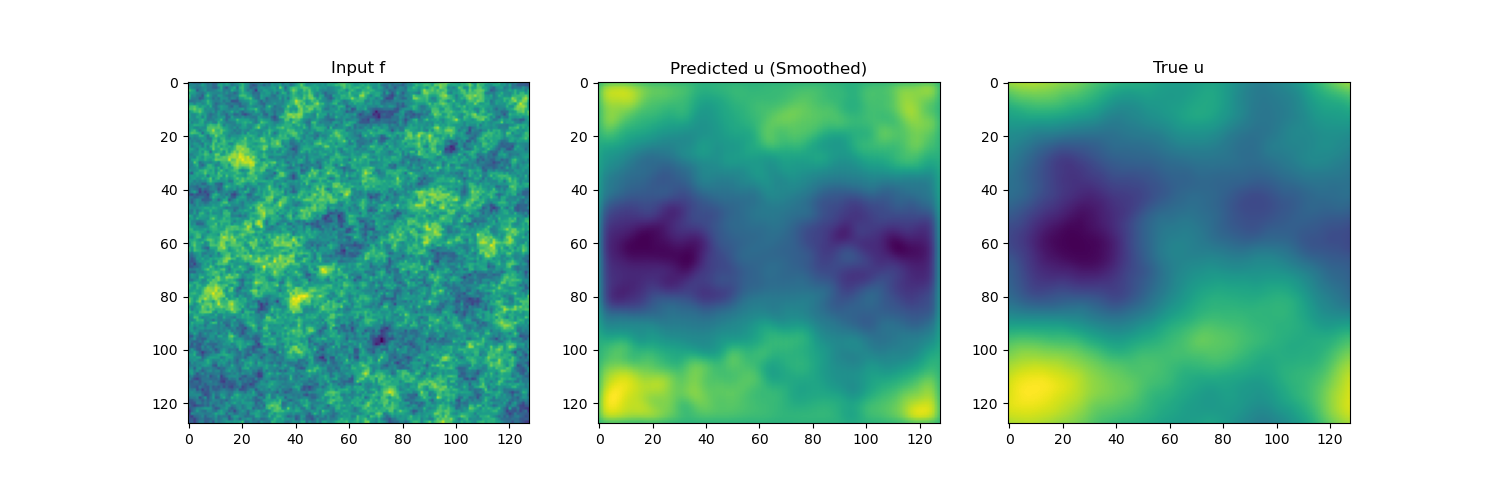
\includegraphics[width=0.6\textwidth]{plot.png}
		\caption{实验数据拟合图}
		\label{fig:1}
	\end{figure}
	
	\section{结论及误差分析}
	根据实验数据处理结果,可以得出以下结论:
	
	\begin{itemize}
		\item [结论1]
		\item [结论2]
		\item [结论3]
	\end{itemize}
	
	在实验过程中,误差主要来源于以下几个方面:
	\begin{enumerate}
		\item [仪器精度误差]
		\item [人为操作误差]
		\item [环境因素误差]
	\end{enumerate}
	
	\section{新发现及讲义中的问题}
	\begin{itemize}
		\item [新发现1]
		\item [新发现2]
		\item [讲义中的问题1]
		\item [讲义中的问题2]
	\end{itemize}
	
	\section{引用源代码}
	在实验中,使用了以下源代码实现数据处理(代码1):
	\lstinputlisting[language=Matlab, caption=数据处理代码]{code.m}
	
	\section{参考文献}
	\begin{thebibliography}{99} % 参考文献编号最多到 99,一般足够
		\bibitem{wang2002新型磁阻传感器在地磁场测量中的应用}
		\textbf{王国余}, \textbf{张欣}, \textbf{景亮}. \emph{新型磁阻传感器在地磁场测量中的应用} [D]. 北京: 清华大学, 2002.
	\end{thebibliography}
	
	
\end{document}
